\section{Techniques used} 

\subsection{Overview}
%Olli
This section describes the techniques that were used to implement the application. Figure \ref{fig:architecture} shows the architecture. The main components are the Chrome browser in which the Chrome extension is installed, a Java server to handle input and output and a set of sources, each of which has its own SPARQL endpoint. 


\begin{figure}[ht]
	\centering
	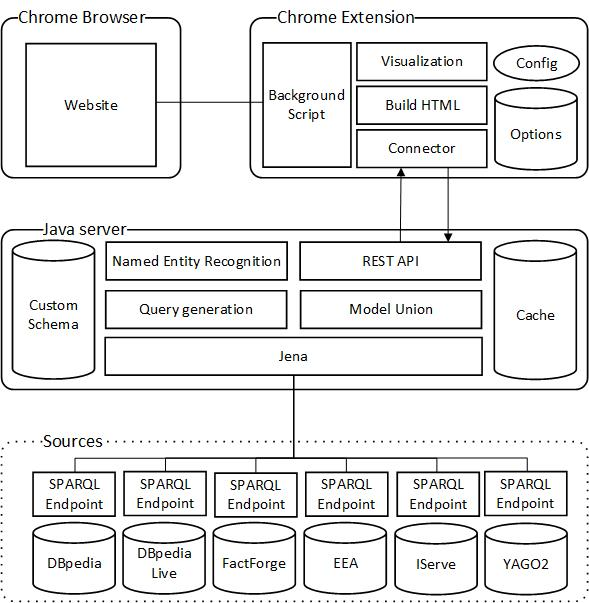
\includegraphics[width=0.8\textwidth]{img/Architecture_v2}
	\caption{Architecture}
	\label{fig:architecture}
\end{figure}


%Reasoning
%Search
%external services
%
%Server
%Chrome extension


\subsection{Named Entity Recognition}
%Olli
Named entity recognition (NER) was used to implement a process that receives as input free text and produces as output a set of named entities based on \cite{NERTutorial}. Stanford's CoreNLP \cite{CoreNLP_NER} was used to implement this. First, the input is cleansed by tokenizing, applying Part-of-Speech tags and lemmatization. Next NER is applied. %OLLI: Ungünstiger Zeilenumbruch

The intermediate result is a set of annotated tokens. To retrieve entities specifically tokens of the type \textit{PERSON}, \textit{LOCATION} and \textit{ORGANIZATION} are used. Other types as described in \cite{CoreNLP_NER} such as \textit{MISC}, \textit{DATE} or \textit{NUMBER} are ignored. The final step is to make sure entities consisting of multiple words, e.g. names, are not retrieved as individual entities. To implement this the tokens are processed sequentially and concatenated as long as they are annotated with the same type. 

For example, the sentence ``Passenger Ruby Gupta, 20, was travelling to Azamagarh to be married on 1 December.'' should produce two entities \texttt{Ruby Gupta} (\textit{PERSON}) and \texttt{Azamagarh} (\textit{LOCATION}) but not an entity \texttt{1 December} (\textit{DATE}). The set of annotated tokens is shown in figure \ref{fig:nerExample}. 

 \begin{figure}[ht]
	\centering
	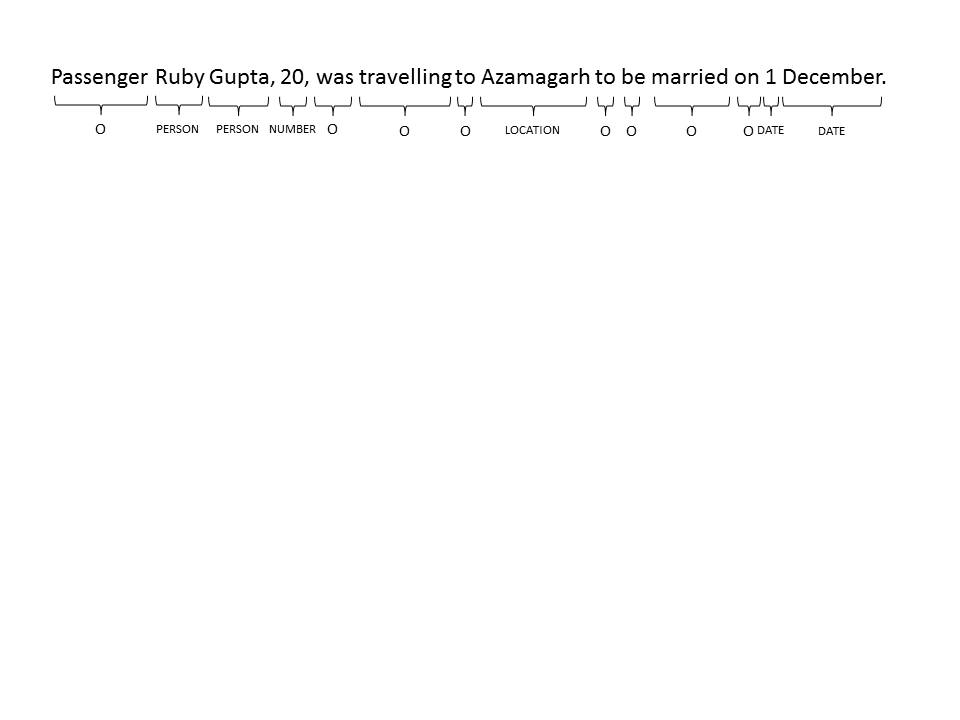
\includegraphics[width=0.8\textwidth]{img/nerExample}
	\caption{Sample NER-annotated text}
	\label{fig:nerExample}
\end{figure}
 




\subsection{SPARQL Queries}
\label{sec:sparqlQueries}
%Sascha
After identifying the named entity and its entity type this information is handed over to the query engine which is implemented using Jena \cite{apache_apache_2016}. The query process is divided into two steps. First all selected sources are queried in parallel. As soon as each query is finished the results are merged into one model. The properties and context triples can be derived from this model. These two steps are illustrated in Figure \ref{fig:details_query} and explained in more detail in the following paragraphs.
\begin{figure}[ht]
	\centering
	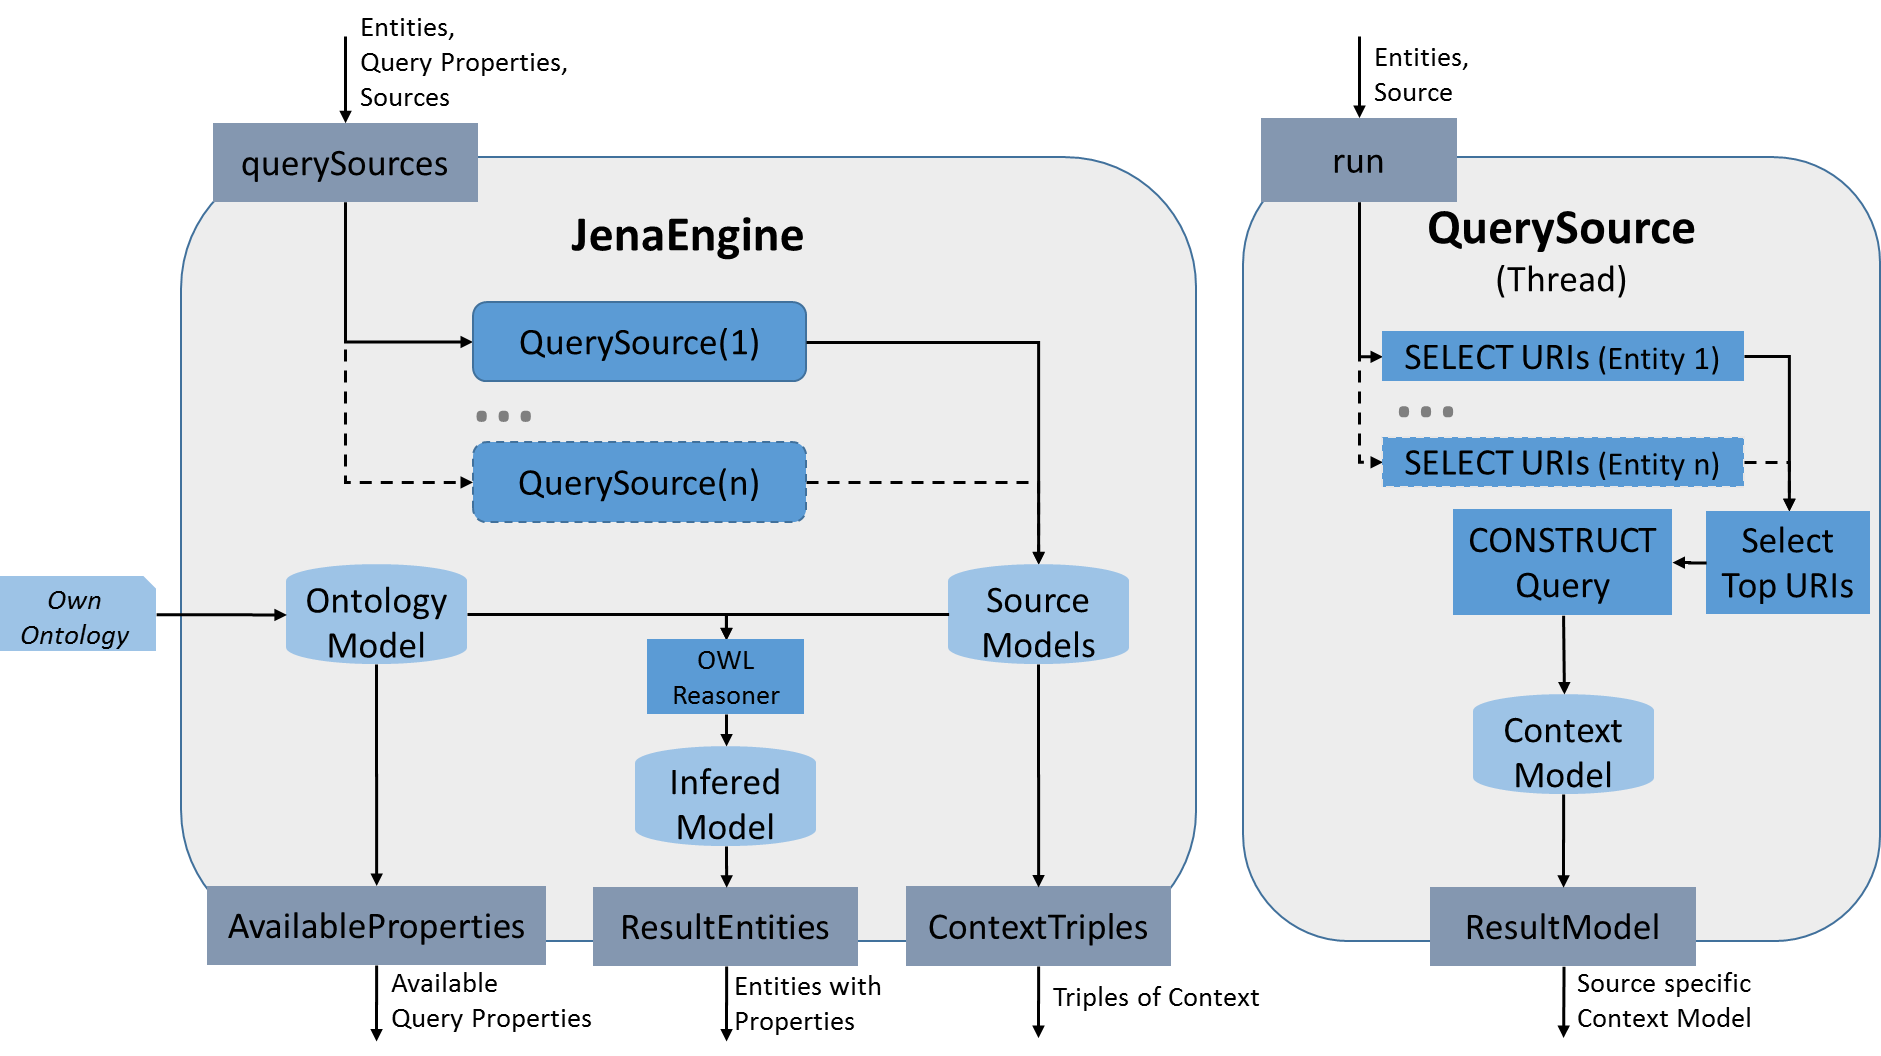
\includegraphics[width=1\textwidth]{img/QueryEngineDetails}
	\caption{Details of Query Engine}
	\label{fig:details_query}
\end{figure}

\paragraph{Querying Sources}
All sources are queried the same way by using the Java class QuerySource as illustrated in Figure \ref{fig:details_query} on the right hand side. Source queries are generalized since the only differences are the endpoint URLs and entity type URIs as described above. An important fact to note is that SPARQL 1.1 functionality like grouping and counting is used. Multiple queries are executed in two steps in order to derive properties and context of a source based on the names and types of the entities.

The first step is the identification of URI candidates by performing a regex based search per identified entity in all selected sources. These queries run in parallel so the system can handle multiple entities without significantly increasing in runtime. Technically multiple \textit{SELECT-Queries} are executed, as shown in Figure \ref{fig:details_query}. The results of these first queries are URIs which meet the type definition and the regex. The regex allows up to 10 characters before and after the identified name. Periods are replaced with ".*" to allow matches with shortened names,  e.g. ''H.* Plattner'' matches ''Hasso Plattner''. In cases there are too many matches (currently the threshold is five), an extended logic is used to reduce the amount of URI candidates. 


The extended logic for URI selection is based on a score which is calculated for each URI by multiplying a \textit{relation score} and the normalized edit distance of the URI label and the entity name. Therefore the source queries provide a count of relations available per URI. This information is used to calculate the \textit{relation score}, which is a relative score, being 1 for the URI with the most relations. The top five URIs with the highest scores are selected. Less URIs are selected if there are not enough URIs having at least a score value of at least 75\% of the highest score value.

This URI identification process is the most expensive in the whole process, because the regex based search of URIs in the sources takes a lot of time. Therefore a cache was introduced which stores the labels per source and entity type for which URIs were already derived. In case a label appears a second time for the same source and entity type, the cached URIs are reused instead of running queries again.


In a second step the identified URI candidates are used to query the source specific context. All properties are queried as well as direct and indirect relations of first order between the entities. Furthermore the labels of all elements are derived as well as OWL \textit{sameAs} relations. 
This query is a \textit{Construct-Query} and therefore returns a model which is the result of the source queries, as shown in Figure \ref{fig:details_query}. 

\paragraph{Custom Ontology}
In order to be able to query properties in a harmonized way across sources and ontologies, a custom ontology was defined for this project. This  ontology mainly consists of OWL \textit{equivelantProperty} definitions for custom properties which group the corresponding sources specific properties. Furthermore there is a mapping of custom classes representing the entity types to the corresponding source specific class definitions of the entities. Therefore the OWL \textit{equivalentClass} property is used. The class definitions are referenced as domains in the properties to specify the applicable entity type. These definitions are stored as an OWL-File\footnote{Stored in repository folder \textit{data}.} which was created initially with WebProtégé \cite{stanford_university_webprotege_2016}, but manually enhanced via a text editor. E.g. property \textit{homepage} is defined as shown below:


\lstset{language=XML,
	morekeywords={encoding,
		owl:ObjectProperty,rdfs:label,rdfs:subPropertyOf,rdfs:domain,owl:equivalentProperty}
}
\tiny
\begin{lstlisting}
<owl:ObjectProperty rdf:about="http://webprotege.stanford.edu/homepage">
	<rdfs:label>homepage</rdfs:label>
	<rdfs:subPropertyOf rdf:resource="http://www.w3.org/2002/07/owl#topObjectProperty"/>
	<rdfs:domain rdf:resource="http://webprotege.stanford.edu/Organisation"/>
	<rdfs:domain rdf:resource="http://webprotege.stanford.edu/Person"/>
	<rdfs:domain rdf:resource="http://webprotege.stanford.edu/Location"/>
	<owl:equivalentProperty rdf:resource="http://xmlns.com/foaf/0.1/homepage"/>
	<owl:equivalentProperty rdf:resource="http://dbpedia.org/property/homepage"/>
	<owl:equivalentProperty rdf:resource="http://dbpedia.org/property/website"/>
	<owl:equivalentProperty rdf:resource="http://xmlns.com/foaf/0.1/page"/>
</owl:ObjectProperty>
\end{lstlisting}
\normalsize



\paragraph{Querying Local Model}
After all source queries are finished the derived models are added to the same local model, as illustrated in Figure \ref{fig:details_query} on the left hand side. This model is combined with the custom ontology described before. For inference the \textit{OWLMicroReasoner} is used. More complex OWL reasoner need much more time, so they are not used for performance reasons. 

Before the properties are derived from this inferred model one URI per entity is derived across sources. The entity with the most relations is chosen. 
For these URIs the properties are then queried based on the custom ontology and are returned as the result. If there are multiple result values for a property all values are returned. If the same value occurs multiple times for the same property, a count is increased. For numeric values additional logic is applied to ensure proper formatting and unit references. All property values including a language tag which is not empty nor English are discarded in order to prevent the texts being shown in multiple languages. As defined before the application focusses on English. 

Furthermore the result context in terms of direct and indirect relations of first order between the entities is returned as well. For the context the original relations are used with there labels, which is outlined in \ref{fig:details_query}. As such relations are returned as well, which are not specified in the custom ontology. 

\subsection{Server} 
\label{sec:server}
%Olli
The server's role in the application is to act as middleware between the frontend and the components that generate and handle SPARQL queries. It implements a REST API with two calls: \textit{GET /RetrieveAvailableProperties} and \textit{POST /RetrieveTriples}. All inputs and outputs are communicated via JSON. The first call is used by the frontend to allow the user to view which attributes are available. The second call retrieves a set of triples for a given text. Examples for both can be viewed in \texttt{README.md}\footnote{Stored in the repository root.}. 

Lastly, the server must implement HTTPS. This is because the user may view websites available only over HTTPS and browsers do not allow mixed content, i.e. loading resources over HTTP on an HTTPS website \cite{ChromeMixedContent}. To achieve this the first idea was to use Heroku for cloud hosting\footnote{\url{https://www.heroku.com/}}. This would ensure that the server is always available and it automatically offers a secure connection. However, it quickly turned out that the server used more memory than was allowed on Heroku (1GB). As such it was decided to use a local server instead. To ensure a secure connection a small server (nginx) with a reverse proxy was used with self signed certificates\cite{nginxReverseProxy}. 




\subsection{Chrome extension}

The Chrome extension handles communication to and from the server and shows the result to the user. It consists mainly of a content script\footnote{\url{https://developer.chrome.com/extensions/content_scripts}}, which is a JavaScript file that is loaded on every website. Upon loading it injects an HTML button that starts the process when clicked. 

\paragraph{Loading triples}
If the user has marked any text on the website this is used as input for the second API call. After the HTTP request has finished loading a popup showing the results is generated and injected into the website. A section is built for each entity showing the triples that were retrieved. Any duplicates are removed. Values with the same relation type (e.g. \textit{abstract}) are compared to each other with the Jaccard similarity measure. If the similarity crosses a threshold the values are hidden as similar attributes. We chose 0.9 as a conservative value that still shows many similar values (particularily \textit{abstract}). The user can view the attributes by clicking on them if he wishes to. We treated further methods of data fusion, such as trying out other similarity measures, as out of scope, as described in the project outline. 


\begin{wrapfigure}{ht}{5.5cm}
  \frame{
	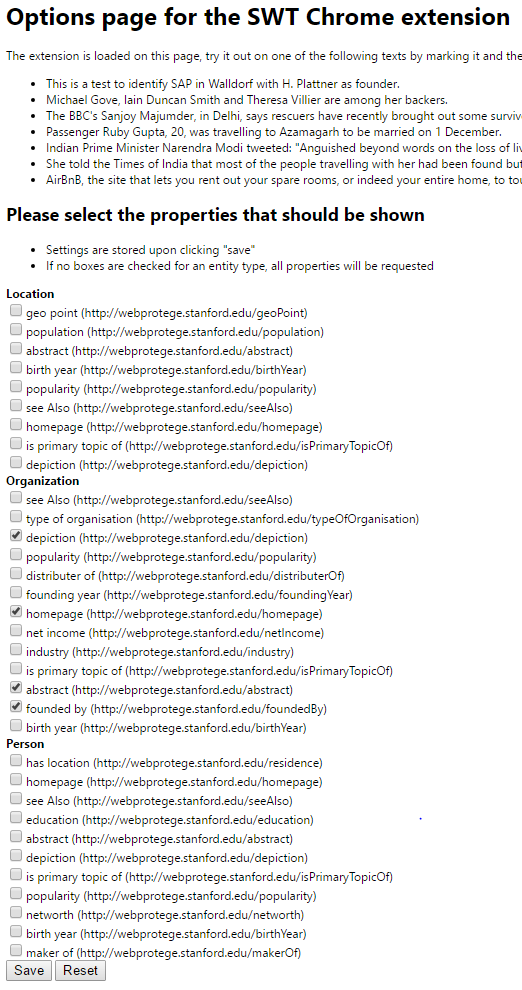
\includegraphics[width=5.5cm]{img/sampleResults/options} %1\textwidth
  }
  \caption{Options page}
  \label{fig:options}
\end{wrapfigure}

\paragraph{Options}
The user has the possibility to customize which attributes are retrieved. For this an options page\footnote{\url{https://developer.chrome.com/extensions/options}} was implemented. This page first loads the available properties via GET /RetrieveAvailableProperties and then shows the results to the user (see figure \ref{fig:options}). The user selects the attributes he is interested in and saves them locally. Any subsequent queries send these options along with the input text. This allows the user to customize the application and reduces bandwidth.

\paragraph{Visualization}
The second API call (\textit{POST /RetrieveTriples}) retrieves the results per named entity and the set of context triples as described in section \ref{sec:sparqlQueries}. These are visualized to show the user the connections between entities. The visualization is generated by D3.js \footnote{\url{https://d3js.org/}} and a force layout. 































